\PassOptionsToPackage{unicode,pdfusetitle}{hyperref}
\PassOptionsToPackage{hyphens}{url}
\PassOptionsToPackage{dvipsnames,svgnames,x11names}{xcolor}

\documentclass[10pt,ignorenonframetext]{beamer}

\usepackage{lmodern}
\usepackage{amssymb,amsmath,mathtools,amsthm}
\usepackage[T1]{fontenc}
\usepackage[utf8]{inputenc}
\usepackage{textcomp} % provide euro and other symbols

\usepackage{pgfpages}

\usepackage{multirow}
\usepackage{csvsimple}
\usepackage{siunitx}

\usepackage{pifont}

% prevent slide breaks in the middle of a paragraph
\widowpenalties 1 10000
\raggedbottom

% Use upquote if available, for straight quotes in verbatim environments
\usepackage{upquote}
\usepackage[]{microtype}
\UseMicrotypeSet[protrusion]{basicmath} % disable protrusion for tt fonts

\usepackage{xcolor}
\usepackage{xurl} % add URL line breaks if available
\usepackage{bookmark}
\usepackage{hyperref}
\hypersetup{%
  colorlinks = true,
  linkcolor  = Cyan4,
  filecolor  = Cyan4,
  citecolor  = SlateBlue4,
  urlcolor   = SlateBlue4
}

% tikz and pgfplots stuff
\usepackage{tikz}
\usetikzlibrary{arrows,shapes,positioning,intersections}
\usepackage{pgfplots}
\usepgfplotslibrary{external,colormaps}
\pgfplotsset{width=7cm,compat=1.11}
%\tikzexternalize

%\usepackage{subfig}
\usepackage{subcaption}
\usepackage{algorithm,algpseudocode}
\usepackage{booktabs}

% bibliography
\usepackage[citestyle=authoryear]{biblatex}
\addbibresource{aistats-slopecd.bib}

\newif\ifbibliography
\setlength{\emergencystretch}{3em} % prevent overfull lines
\setcounter{secnumdepth}{-\maxdimen} % remove section numbering


% redefine part, section, and subsection headers

\raggedbottom
\setbeamertemplate{part page}{
  \centering
  \begin{beamercolorbox}[sep=16pt,center]{part title}
    \usebeamerfont{part title}\insertpart\par
  \end{beamercolorbox}
}
\setbeamertemplate{section page}{
  \centering
  \begin{beamercolorbox}[sep=12pt,center]{part title}
    \usebeamerfont{section title}\insertsection\par
  \end{beamercolorbox}
}
\setbeamertemplate{subsection page}{
  \centering
  \begin{beamercolorbox}[sep=8pt,center]{part title}
    \usebeamerfont{subsection title}\insertsubsection\par
  \end{beamercolorbox}
}

\AtBeginPart{\frame{\partpage}}
\AtBeginSection{\ifbibliography\else\frame{\sectionpage}\fi}
\AtBeginSubsection{\frame{\subsectionpage}}

% beamer configuration
\usecolortheme{dove}
\usefonttheme{professionalfonts}
\usefonttheme{structurebold}
\setbeamertemplate{footline}[frame number]
\setbeamertemplate{caption}[numbered]
\setbeamertemplate{caption label separator}{: }
\setbeamercolor{caption name}{fg=normal text.fg}
\setbeamertemplate{frametitle}{%
  \begin{centering}\insertframetitle\par\end{centering}%
}
\setbeamertemplate{itemize item}{\(\bullet\)}
%\setbeamertemplate{itemize item}[circle]
\setbeamertemplate{itemize subitem}{\(\circ\)}
\setbeamertemplate{itemize subsubitem}{\textendash}
\setbeamerfont{frametitle}{size=\large}
\setbeamertemplate{headline}{\vskip5ex}
\beamertemplatenavigationsymbolsempty
%\setlength{\parskip}{1em} % add paragraph spacing



% operators
\DeclareMathOperator*{\argmax}{arg\,max}
\DeclareMathOperator*{\argmin}{arg\,min}
\DeclareMathOperator{\E}{\text{E}}
\DeclareMathOperator{\var}{var}
\DeclareMathOperator{\cov}{cov}
\DeclareMathOperator{\sign}{sign}
\DeclareMathOperator{\card}{card}
\DeclareMathOperator{\cumsum}{cumsum}
\DeclareMathOperator*{\prox}{prox}

% macros
\newcommand{\pkg}[1]{\textsf{#1}}
\renewcommand{\vec}{\vectorsym}
\newcommand{\mat}{\matrixsym}
\newcommand{\du}{\mathrm{d}}

\makeatletter
\newcommand\notsotiny{\@setfontsize\notsotiny\@vipt\@viipt}
\makeatother



% title block
\title{Coordinate Descent for SLOPE}
\author[shortname]{\alert{Johan Larsson}\inst{1} \and Quentin Klopfenstein\inst{2,3} \and Mathurin Massias\inst{3,4} \and Jonas Wallin\inst{1}}
\institute[shortinst]{
  \inst{1}{Department of Statistics, Lund University}
  \inst{2}{Luxembourg Centre for Systems Biomedicine}
  \inst{3}{University of Luxembourg, Luxembourg}
  \inst{4}{University of Lyon, Inria, CNRS, ENS de Lyon}
  \inst{5}{UCB Lyon 1, LIP UMR 5668, F-69342}
}
\date{\today}
\titlegraphic{%
  \hfill
  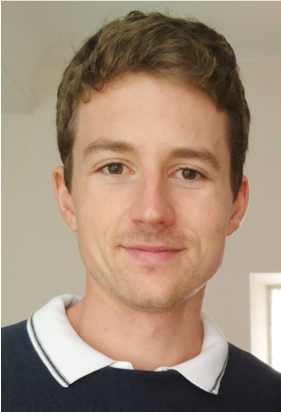
\includegraphics[height=2cm]{figures/quentin.png}
  \hfill
  
\includegraphics[height=2cm]{figures/mathurin.jpg}
  \hfill
  
\includegraphics[height=2cm]{figures/jonas.jpg}
  \hfill
  \null
}

\begin{document}
\frame[noframenumbering,plain]{\titlepage}

\begin{frame}[c]
  \frametitle{Synopsis}

  \begin{block}{The Problem}
    SLOPE is a sparsity-inducing model with appealing properties, but the
    best algorithms (up til now) for solving SLOPE are slow.

    \begin{block}{Our Contribution}
      A hybrid algorithm based on coordinate descent and
      proximal gradient descent.
    \end{block}
  \end{block}

\end{frame}

\begin{frame}
  \frametitle{Sorted L-One Penalized Estimation (SLOPE)}

  For a design matrix \(X \in \mathbb{R}^{n \times p}\) and response vector \(y \in \mathbb{R}^n\), the solution to SLOPE is
  \[
    \beta^* \in \argmin_{\beta \in \mathbb{R}^p}
    \left\{P(\beta) =  \frac{1}{2} \norm{y - X \beta}^2 + J(\beta)\right\}
  \]
  where
  \begin{equation*}
    \label{eq:sorted-l1-norm}
    J(\beta) = \sum_{j=1}^p \lambda_j|\beta_{(j)}|
  \end{equation*}
  is the \alert{sorted \(\ell_1\) norm}, defined through
  \begin{equation}
    |\beta_{(1)}| \geq |\beta_{(2)}| \geq \cdots \geq |\beta_{(p)}|,
  \end{equation}
  with \(\lambda\) being a fixed non-increasing and non-negative sequence.

  \pause

  \begin{block}{Generalizations}
    \begin{itemize}
      \item \(\lambda_1 = \cdots = \lambda_p \rightarrow \ell_1\) (the lasso penalty)
      \item \(\lambda_1 > \lambda_2 = \cdots = \lambda_p = 0 \rightarrow \ell_\infty\)
    \end{itemize}
  \end{block}

\end{frame}

\begin{frame}[c]
  \frametitle{Properties}

  \begin{columns}
    \begin{column}{0.45\textwidth}
      \begin{itemize}
        \item \alert{Clustering}~\parencite{bogdan2022,schneider2020a,figueiredo2016}
        \item \alert{Control of false discovery rate}~\parencite{bogdan2013,bogdan2015}
        \item \alert{Recovery of sparsity and ordering patterns}~\parencite{bogdan2022}
        \item \alert{Convexity}
      \end{itemize}

    \end{column}
    \begin{column}{0.45\textwidth}
      \begin{figure}
        \centering
        \pgfplotsset{width=6cm,height=6cm}
        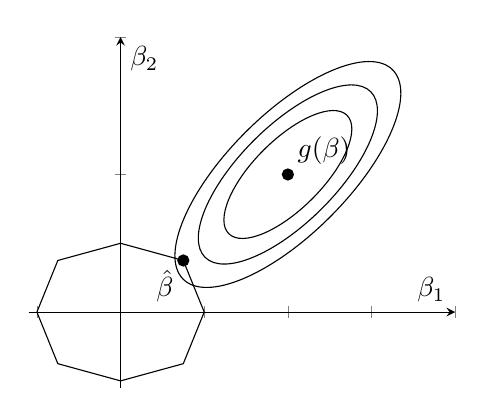
\begin{tikzpicture}
\begin{axis}[
    xlabel = \(\beta_1\),
    ylabel = \(\beta_2\),
    ymin = -1.1,
    ymax = 4,
    xmin = -1.1,
    xmax = 4,
    axis lines = center,
    yticklabels={,,},
    xticklabels={,,}
]
\draw[rotate around={45:(2,2)}] (2,2) ellipse (1 and 0.5);
\draw[rotate around={45:(2,2)}] (2,2) ellipse (1.4 and 0.7);
\draw[rotate around={45:(2,2)}] (2,2) ellipse (1.77 and 0.87);

\addplot[]
    coordinates {
    	(-1,0)
    	(-0.75, 0.75)
    	(0,1)
    	(0.75,0.75)
    	(1,0)
    	(0.75,-0.75)
    	(0,-1)
    	(-0.75,-0.75)
    	(-1,0)
    };
\addplot [only marks, mark=*] coordinates {(2,2)};
\node [above right,black] at (2,2) {$g(\beta)$};

\addplot [only marks, mark=*] coordinates { (0.75,0.75) };
\node [below left] at (0.75,0.75) {$\hat\beta$};
\end{axis}
\end{tikzpicture}
        \caption{%
          The SLOPE solution seen as a constrained problem.
        }
        \label{fig:slope-solution}
      \end{figure}

    \end{column}
  \end{columns}

\end{frame}

\begin{frame}[c]
  \frametitle{Why Does Not Everyone Use SLOPE?}
  % \framesubtitle{Why doesn't everyone already use SLOPE?}

  \begin{columns}
    \begin{column}{0.45\textwidth}
      \begin{itemize}
        \item<1-> The lasso is much more popular than SLOPE.
        \item<2-> One reason is that current state-of-the-art algorithms for fitting the lasso are faster.
        \medskip

        \textbf{Example}: Fitting the \texttt{bcTCGA} data set with the R-package SLOPE takes
        43 seconds versus 0.14 seconds for glmnet (lasso).
      \end{itemize}

    \end{column}
    \begin{column}{0.45\textwidth}
      \begin{figure}
        \centering
        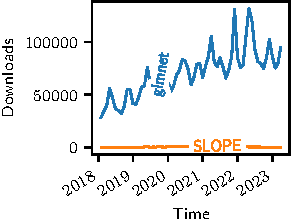
\includegraphics[]{figures/cran-stats.pdf}
        \caption{%
          CRAN download statistics for the SLOPE and glmnet (lasso) packages.
        }
        \label{fig:cran-stats}
      \end{figure}
    \end{column}
  \end{columns}
\end{frame}

\begin{frame}
  \frametitle{Coordinate Descent}

  \begin{columns}[c]
    \begin{column}{0.45\textwidth}

      \begin{itemize}
        \item<1-> Coordinate descent (CD) works great for the lasso~\parencite{friedman2010}.
        \item<2->
        Unfortunately, we cannot directly use CD for SLOPE since the
        sorted \(\ell_1\) norm is \alert{not separable}:
        \[
          J(\beta) = \sum_{j=1}^p \lambda_j |\beta_{(j)}|.
        \]
      \end{itemize}

      \medskip

    \end{column}
    \begin{column}{0.45\textwidth}
      \begin{figure}[htpb]
        \centering
        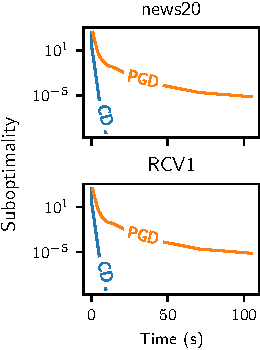
\includegraphics[]{figures/cd-vs-pgd.pdf}
        \caption{%
          Coordinate descent versus proximal gradient descent for the lasso.
        }
        \label{fig:cd-vs-pgd}
      \end{figure}
    \end{column}
  \end{columns}

\end{frame}

\begin{frame}
  \frametitle{The SLOPE Problem is Not Separable}

  \begin{figure}[htpb]
    \centering
    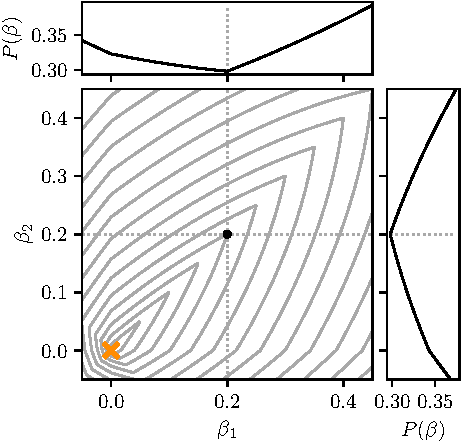
\includegraphics[scale=0.8]{figures/naive-cd-stuck.pdf}
    \caption{A \emph{naive} coordinate descent algorithm cannot advance from the
      current iterate (\ding{108}) to reach the optimum ({\color{orange}\ding{54}}).}
    \label{fig:naive-cd}
  \end{figure}
\end{frame}

\begin{frame}[c]
  \frametitle{Clusters Are Not Known In Advance}

  If the clusters were known, the problem would become separable,
  \[
    \min_{z \in \mathbb{R}^{m^*}}\bigg(
    \frac{1}{2} \Big\lVert y - X \sum_{i=1}^{m^*} \sum_{j \in \mathcal{C}_i^*} z_i \sign(\beta_j^*) e_j \Big\rVert^2 + \sum_{i=1}^{m^*} | z_i | \sum_{j \in \mathcal{C}_i^*} \lambda_j
    \bigg),
  \]
  and we could solve it using CD.

  \pause

  \begin{block}{Idea}
    Alternate between gradient descent steps that identify the clusters
    (via partial smoothness) and
    coordinate descent steps \alert{on the clusters}, which enable fast convergence.
  \end{block}

\end{frame}

\begin{frame}[c]
  \frametitle{Hybrid Algorithm}

  \begin{itemize}
    \item Every \(v\)th iteration, take a full proximal gradient step.
          This allows clusters to split (or merge).
    \item At all other iterations, take coordinate descent steps on the clusters.
  \end{itemize}

  \pause

  \begin{figure}[htpb]
    \centering
    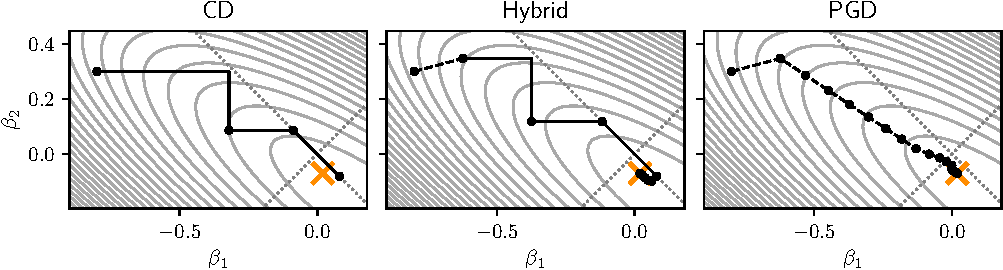
\includegraphics[width=\textwidth]{figures/illustration_solvers.pdf}
    \caption{%
      Our algorithm (hybrid) is a combination of CD and PGD.
    }
    \label{fig:illustration}
  \end{figure}

\end{frame}

\begin{frame}
  \frametitle{Coordinate Descent Steps}

  When updating the \(k\)th cluster, we let
  \begin{equation*}
    \beta_i(z) =
    \begin{cases}
      \mathrm{sign}(\beta_i) z   , & \text{if } i \in \mathcal{C}_k, \\
      \beta_i,                     & \text{otherwise}.
    \end{cases}
  \end{equation*}

  \pause

  Minimizing the objective in this direction amounts to solving the following
  one-dimensional problem:
  \[
    \min_{z \in \mathbb{R}} \Big(
    G(z) = P(\beta(z))  = \frac{1}{2} \lVert y - X \beta(z)\rVert^2 + H(z)
    \Big),
  \]
  where
  \begin{equation*}
    H(z) = |z| \sum_{j \in \mathcal{C}_k} \lambda_{(j)^-_z}
    + \sum_{j \notin \mathcal{C}_k} |\beta_j| \lambda_{(j)^-_z}
  \end{equation*}
  is the \emph{partial sorted \(\ell_1\) norm} with respect to the \(k\)-th cluster and where we write \(\lambda_{(j)^-_z}\) to indicate that the inverse sorting permutation \((j)^-_z\)
  is defined with respect to \(\beta(z)\).
\end{frame}

\begin{frame}
  \frametitle{The Partial Sorted \(\ell_1\) Norm}

  \begin{figure}[htpb]
    \centering
    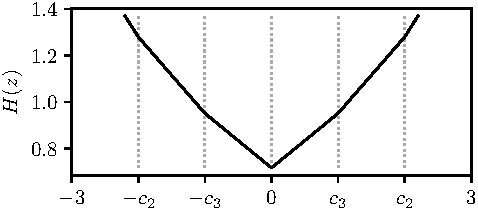
\includegraphics[scale=0.8]{figures/partial_slope.pdf}
    \caption{%
    The partial sorted \(\ell_1\) norm with \(\beta = [-3,1,3,2]^T\), \(k = 1\), and so
    \(c_1, c_2, c_3 = (3,2,1)\).
    }
    \label{fig:partial-sl1}
  \end{figure}
\end{frame}

\begin{frame}
  \frametitle{How Do We Minimize Over One Cluster?}

  \begin{columns}
    \begin{column}{0.45\textwidth}
      The optimality condition, using the directional derivative, is
      \[
        \forall \delta \in \{-1, 1\}, \quad G'(z; \delta) \geq 0,
      \]
      with
      \[
        \begin{multlined}
          G'(z; \delta)  \\= \delta \sum_{j \in \mathcal{C}_k} X_{:j}^\top(X\beta(z) - y) \\
          + H'(z; \delta).
        \end{multlined}
      \]
    \end{column}
    \begin{column}{0.45\textwidth}
      \begin{figure}
        \centering
        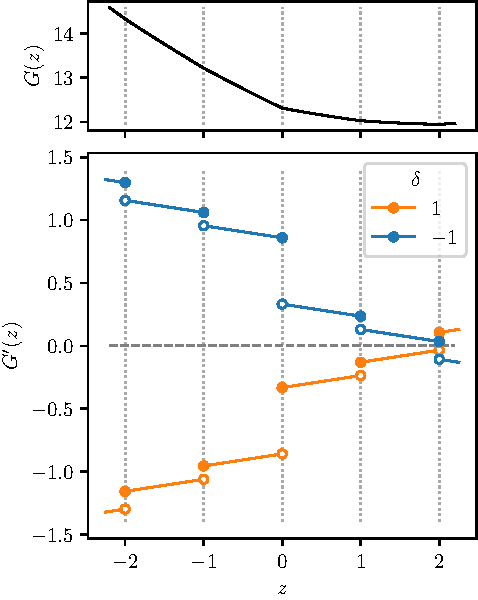
\includegraphics[width=\textwidth]{figures/directional-derivative.pdf}
        \caption{%
        \(G\) and its directional derivative \(G'( \cdot ; \delta)\) for
        an example with \(\beta = [-3, 1, 3, 2]^T\), \(k = 1\), and consequently
        \(c^{\setminus k} = \{1, 2\}\).
        }
        \label{fig:}
      \end{figure}
    \end{column}
  \end{columns}
\end{frame}

\begin{frame}
  \frametitle{The SLOPE Thresholding Operator}

  \begin{figure}[htpb]
    \centering
    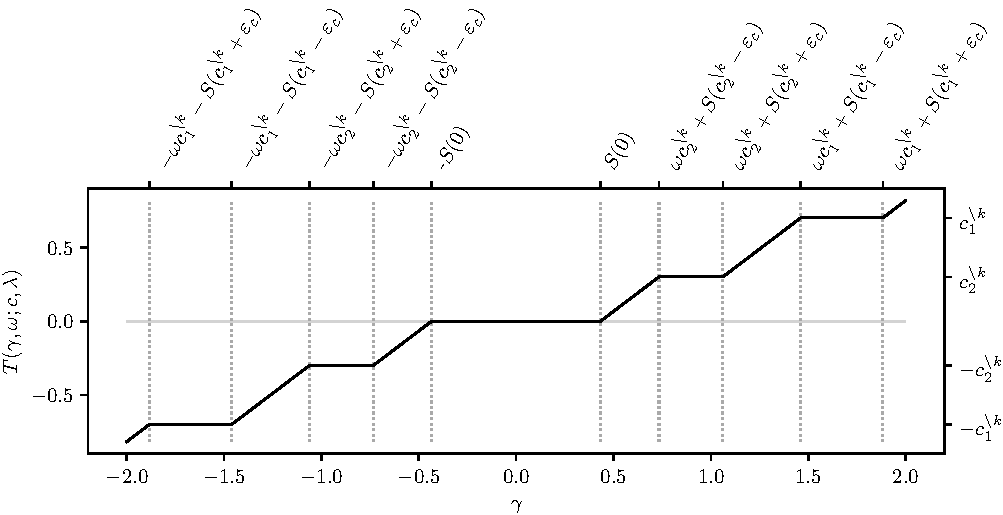
\includegraphics[width=\textwidth]{figures/slope-thresholding.pdf}
    \caption{%
      The SLOPE Thresholding Operator
    }
    \label{fig:thresholding-operator}
  \end{figure}
\end{frame}

\begin{frame}
  \frametitle{Experiments}
  \framesubtitle{Real Data}

  \begin{figure}[htpb]
    \centering
    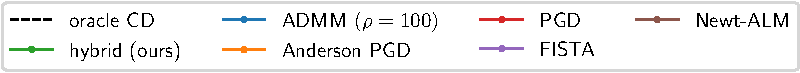
\includegraphics[scale=0.55]{figures/real_legend.pdf}
    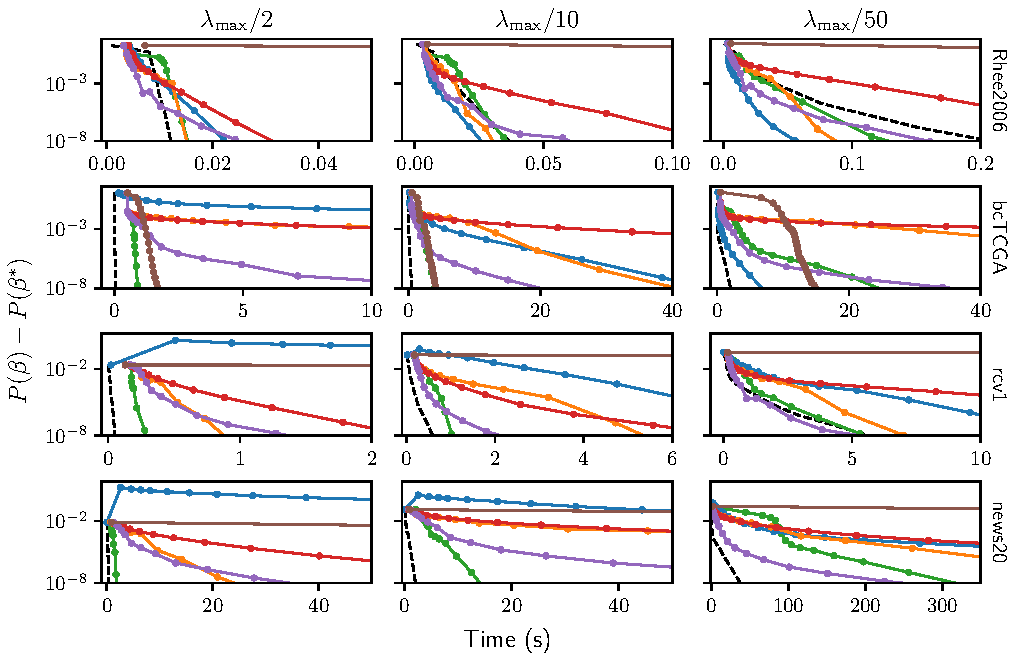
\includegraphics[scale=0.55]{figures/real.pdf}
    \caption{%
      Benchmarks on real data
    }
  \end{figure}
\end{frame}

\begin{frame}
  \frametitle{Experiments}
  \framesubtitle{Simulated Data}

  \begin{figure}[htpb]
    \centering
    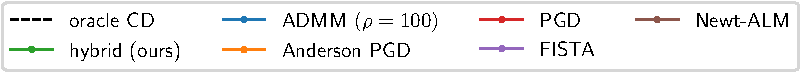
\includegraphics[scale=0.55]{figures/simulated_legend.pdf}
    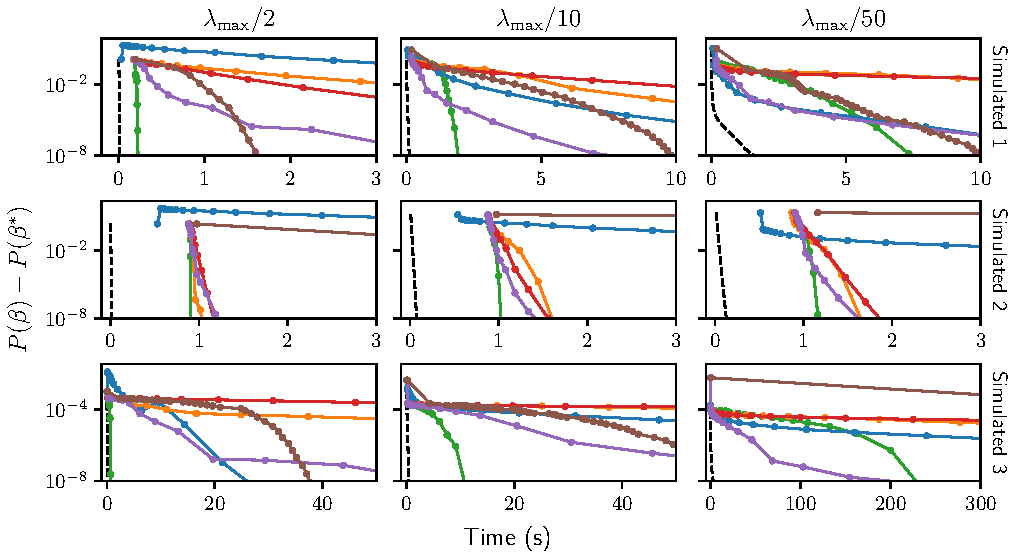
\includegraphics[scale=0.6]{figures/simulated.pdf}
    \caption{%
      Benchmarks on simulated data. Scenario 1: \(n = 200\) and \(p = 20\,000\), 
      \(X\). Scenario 2: \(n = 20\,000\) and \(p = 200\). Scenario 3: \(n = 200\), 
      \(p = 200\,000\), and sparse \(X\).
    }
  \end{figure}
\end{frame}

\begin{frame}[c]
  \frametitle{Wrap Up}

  \begin{itemize}
    \item Experiments were set up using
          Benchopt (\href{https://benchopt.github.io}{\texttt{benchopt.github.io}})
    \item Code is available at
          \href{https://github.com/jolars/slopecd}{\texttt{github.com/jolars/slopecd}}
    \item Add your own solver for SLOPE at
          \href{https://github.com/benchopt/benchmark\_SLOPE}{\texttt{github.com/benchopt/benchmark\_SLOPE}}
  \end{itemize}

  \vfill\hfill
  
\includegraphics[width=0.5\textwidth]{figures/benchopt_logo.pdf}
\end{frame}

\begin{frame}[allowframebreaks]{References}
  \bibliographytrue
  \printbibliography[heading=none]
\end{frame}

\end{document}
